
\pdfminorversion=4 % for acroread
\documentclass[aspectratio=169,t,xcolor={usenames,dvipsnames}]{beamer}
%\documentclass[t,handout,xcolor={usenames,dvipsnames}]{beamer}
\usepackage{../beamerstyle}
\usepackage{dsfont}
\usepackage{bm}
\usepackage[english]{babel}
\usepackage[utf8]{inputenc}
\usepackage{graphicx}
\usepackage{algorithm}
\usepackage[ruled,vlined,algo2e,linesnumbered]{algorithm2e}
%\usepackage[boxed,vlined]{algorithm2e}
\usepackage{hyperref}
\usepackage{booktabs}
\usepackage{mathtools}

\usepackage{amsmath,amssymb}
\usepackage{listings}
\lstset{frame=lines,framesep=3pt,numbers=left,numberblanklines=false,basicstyle=\ttfamily\small}

\usepackage{subfig}
\usepackage{multicol}
%\usepackage{appendixnumberbeamer}
%
\usepackage{tcolorbox}

\usepackage{pgfplots}
\usepackage{tikz}
\usetikzlibrary{trees} 
\usetikzlibrary{shapes.geometric}
\usetikzlibrary{positioning,shapes,shadows,arrows,calc,mindmap}
\usetikzlibrary{positioning,fadings,through}
\usetikzlibrary{decorations.pathreplacing}
\usetikzlibrary{intersections}
\usetikzlibrary{positioning,fit,calc,shadows,backgrounds}
\pgfdeclarelayer{background}
\pgfdeclarelayer{foreground}
\pgfsetlayers{background,main,foreground}
\tikzstyle{activity}=[rectangle, draw=black, rounded corners, text centered, text width=8em]
\tikzstyle{data}=[rectangle, draw=black, text centered, text width=8em]
\tikzstyle{myarrow}=[->, thick, draw=black]

% Define the layers to draw the diagram
\pgfdeclarelayer{background}
\pgfdeclarelayer{foreground}
\pgfsetlayers{background,main,foreground}

%\usepackage{listings}
%\lstset{numbers=left,
%  showstringspaces=false,
%  frame={tb},
%  captionpos=b,
%  lineskip=0pt,
%  basicstyle=\ttfamily,
%%  extendedchars=true,
%  stepnumber=1,
%  numberstyle=\small,
%  xleftmargin=1em,
%  breaklines
%}

 
\definecolor{blue}{RGB}{0, 74, 153}

\usetheme{Boadilla}
%\useinnertheme{rectangles}
\usecolortheme{whale}
\setbeamercolor{alerted text}{fg=blue}
\useoutertheme{infolines}
\setbeamertemplate{navigation symbols}{\vspace{-5pt}} % to lower the logo
\setbeamercolor{date in head/foot}{bg=blue} % blue
\setbeamercolor{date in head/foot}{fg=white}
\setbeamercolor{author in head/foot}{bg=blue} %blue
\setbeamercolor{title in head/foot}{bg=blue} % blue
\setbeamercolor{title}{fg=white, bg=blue}
\setbeamercolor{block title}{fg=white,bg=blue}
\setbeamercolor{block body}{bg=blue!10}
\setbeamercolor{frametitle}{fg=white, bg=blue}
\setbeamercovered{invisible}

\makeatletter
\setbeamertemplate{footline}
{
  \leavevmode%
  \hbox{%
  \begin{beamercolorbox}[wd=.333333\paperwidth,ht=2.25ex,dp=1ex,center]{author in head/foot}%
    \usebeamerfont{author in head/foot}\insertshortauthor
  \end{beamercolorbox}%
  \begin{beamercolorbox}[wd=.333333\paperwidth,ht=2.25ex,dp=1ex,center]{title in head/foot}%
    \usebeamerfont{title in head/foot}\insertshorttitle
  \end{beamercolorbox}%
  \begin{beamercolorbox}[wd=.333333\paperwidth,ht=2.25ex,dp=1ex,right]{date in head/foot}%
    \usebeamerfont{date in head/foot}Week \@week, Topic \@topicnumber, Slide \insertframenumber{}\hspace*{2em}
%    \insertframenumber\hspace*{2ex} 
  \end{beamercolorbox}}%
  \vskip0pt%
}

\newcommand{\@week}{0}
\newcommand{\@topicnumber}{0}
\newcommand{\week}[1]{\renewcommand{\@week}{#1}}
\newcommand{\topicnumber}[1]{\renewcommand{\@topicnumber}{#1}}

\makeatother

%\pgfdeclareimage[height=1.2cm]{automl}{images/logos/automl.png}
%\pgfdeclareimage[height=1.2cm]{freiburg}{images/logos/freiburg}

%\logo{\pgfuseimage{freiburg}}

\input{../latex_main/macros}





\title[AutoML: Overview]{AutoML: Algorithm Selection} % week title
\subtitle{Algorithm Selection} % video title
\author[Lars Kotthoff]{Bernd Bischl \and Frank Hutter \and \underline{Lars Kotthoff}\newline \and Marius Lindauer \and Joaquin Vanschoren}
\institute{}
\date{}
\week{3}
\topicnumber{2}



% \AtBeginSection[] % Do nothing for \section*
% {
%   \begin{frame}{Outline}
%     \bigskip
%     \vfill
%     \tableofcontents[currentsection]
%   \end{frame}
% }

\begin{document}
	
	\maketitle
	

\begin{frame}[c]{Algorithm Selection}
\begin{center}
\resizebox{.7\textwidth}{!}{%
\tikzset{>=latex}
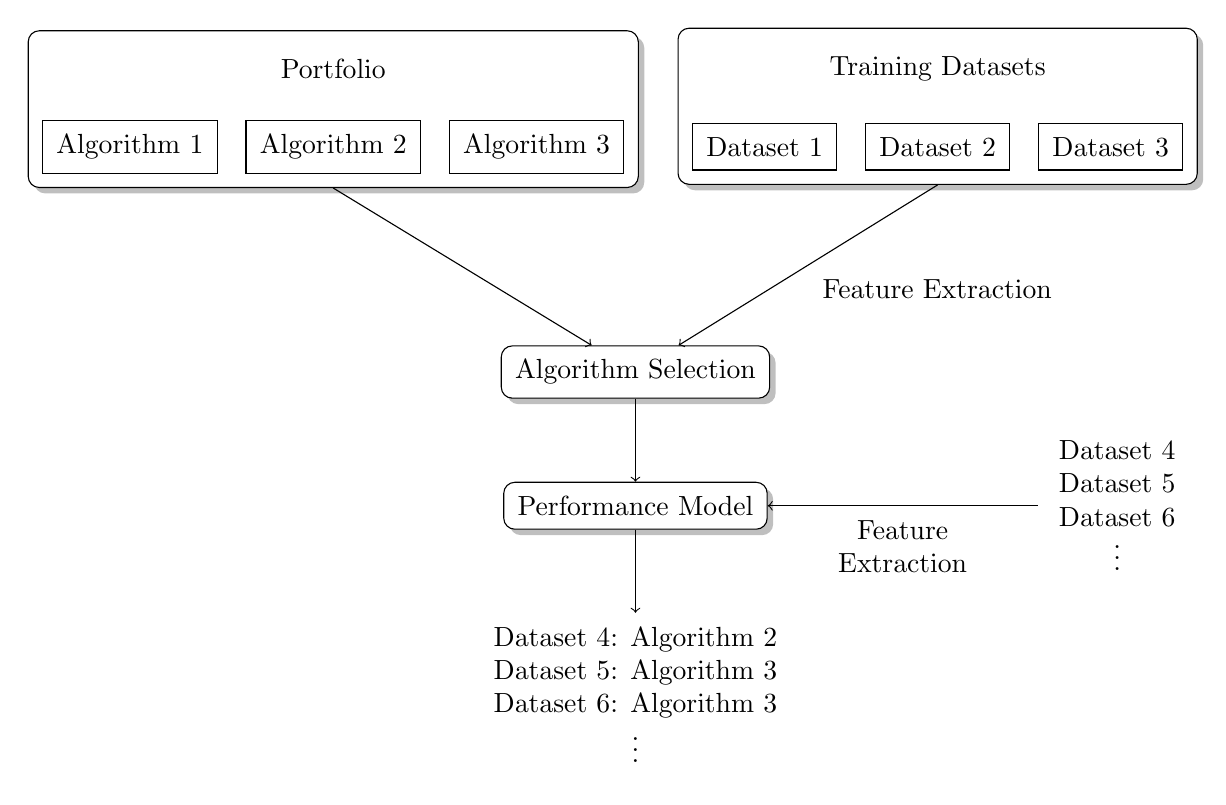
\begin{tikzpicture}[node distance=1em,inner sep=.5em,n/.style={drop
shadow,fill=white,rounded corners},scale=.5]
\node (p) [align=left] {Portfolio};
\node (a2) [rectangle,align=center,below=of p,draw] {Algorithm 2};
\node (a1) [rectangle,align=center,left=of a2,draw] {Algorithm 1};
\node (a3) [rectangle,align=center,right=of a2,draw] {Algorithm 3};
\begin{pgfonlayer}{background}
\node (pc) [n,fit={(p) (a1) (a2) (a3)},draw] {};
\end{pgfonlayer}

\node (i) [align=left,right=15em of p.east] {Training Datasets};
\node (i2) [rectangle,align=center,below=of i,draw] {Dataset 2};
\node (i1) [rectangle,align=center,left=of i2,draw] {Dataset 1};
\node (i3) [rectangle,align=center,right=of i2,draw] {Dataset 3};
\begin{pgfonlayer}{background}
\node (ic) [n,fit={(i) (i1) (i2) (i3)},draw] {};
\end{pgfonlayer}

\node (as) [n,draw,align=left,below=10em of $(p)!0.5!(i)$] {Algorithm Selection};
\node (m) [n,draw,align=left,below=3em of as] {Performance Model};

\node (it) [align=center,right=10em of m] {Dataset 4\\Dataset 5\\Dataset 6\\$\vdots$};

\node (s) [align=center,below=3em of m] {Dataset 4: Algorithm 2\\Dataset 5: Algorithm 3\\Dataset 6: Algorithm 3\\$\vdots$};

\path [->] (pc.south) edge (as);
\path [->] (ic.south) edge node [below right] {Feature Extraction} (as);
\path [->] ([xshift=-.5em]it.west) edge node [below,align=center] {Feature\\Extraction} (m.east);
\path [->] (as.south) edge (m.north);
\path [->] (m.south) edge (s.north);
\end{tikzpicture}}
\end{center}
\end{frame}

\begin{frame}[c]{Algorithm Portfolios}
\begin{itemize}
    \item instead of a single algorithm, use several (hopefully complementary) algorithms
\item idea from Economics -- minimize risk by spreading it out across several
    securities
\item same here -- minimize risk of algorithm performing poorly
\item in practice often constructed from algorithms known to perform well
\item idea similar to ensembles or boosting -- leverage strengths and alleviate
    weaknesses, but learn which algorithm to choose for a particular dataset
\end{itemize}
\end{frame}

\begin{frame}[c]{Algorithms}
``algorithm'' used in a very loose sense
\begin{itemize}
\item different learners
\item different parameterizations of the same learner
\item different ensembles, boosted learners
\item different machine learning workflows/pipelines
\item \ldots
\end{itemize}
\end{frame}

\begin{frame}[c]{Evaluation of Portfolios}
\begin{itemize}
\item single best algorithm
    \begin{itemize}
    \item algorithm with the best performance across all datasets
    \item lower bound for performance of portfolio -- hopefully we are better!
    \end{itemize}
\item virtual best algorithm
    \begin{itemize}
    \item choose the best algorithm for each dataset
    \item corresponds to oracle predictor or overhead-free parallel portfolio
    \item upper bound on portfolio performance
    \end{itemize}
\end{itemize}
\end{frame}

\begin{frame}[c]{Parallel Portfolios}
Why not simply run all algorithms in parallel?
\begin{itemize}
\item not enough resources may be available/waste of resources
\item algorithms may be parallelized themselves
\item memory contention
\item \ldots
\end{itemize}
\end{frame}

\begin{frame}[c]{Building an Algorithm Selection System}
\begin{itemize}
    \item most approaches rely on (meta-)machine learning
\item train with representative data, i.e.\ performance of all algorithms in
    portfolio on representative datasets
\item evaluate performance on separate set of datasets
\item potentially large amount of prep work
\item existing repositories of machine learning performances (e.g. OpenML) can
    help
\end{itemize}
\end{frame}

\begin{frame}[c]{Choosing Datasets}
\begin{itemize}
\item we want selectors that generalize, i.e.\ good for more than one
dataset
\item split datasets into training set (which we learn a selector on) and test set
(which we only evaluate performance on)
\item need to balance easy/hard datasets in both sets
\item may need a lot of data
\end{itemize}
\end{frame}

\begin{frame}[c]{Key Components of an Algorithm Selection System}
\begin{itemize}
\item feature extraction
\item performance model
\item prediction-based selector
\end{itemize}
optional:
\begin{itemize}
\item presolver
\item secondary/hierarchical models and predictors (e.g.\ for feature extraction
    time to avoid spending a long time for small performance gains)
\end{itemize}
\end{frame}

\end{document}
